\section{Pimental}



\subsection*{Observed experimental dynamics}

Pimentel et al. devised and ran an experiment in which two populations of flies are pitted against each other in a fight for domination and ultimately, survival. \cite{pimentel1965selection}
\cite{hutchingson2018ecological} Suppose you placed a colony of houseflies (Musca Domestica) in one side of a boxed enclosure; a competing number of Blowflies (Phaenicia) at the other. What would eventually happen given an ample but finite supply of food to the container? Before long you would see a niche domination by one of the species. The arrangement being unstable, either the house or blow fly population would eventually see-off the other.\par
Pimentel and his colleagues did something clever to augment the dynamics of this experiment: they contrived an enclosure, take the original box, but with a myriad of internal sub-compartments. A kind of three-dimensional maze of tunnels and mini chambers. Such arrangement permits a desirable property to the enclosure -- with the populations initially placed at opposing sides, eventual communication by contact, interaction is delayed by a period greater than the average lifespan of either species. That is, in the months taken for the dissipation of a species from one side to the other, multiple generations ensue. But why is this desirable?\par
By slowing the potential spread of the species, Pimentel introduces the constraint that given a total domination is arrived at, it can not be won in a time of only one or a few fly lifespans. The war must be won over succeeding generations; grandchildren's grandchildren, all fighting for the same cause. And this allows for the hand of Darwinian selection to come into play.\par
An observation of this contrivance saw the following dynamic. Blowflies were pushed almost to extinction by the initially superior abounding of Musca Domestica, but then, the tides turned... From the brink, the blowfly under-dogs managed to claw back their footing and eventually overthrow the advances of their adversaries.\par
It is hypothesised that during this squeeze of reduced population, the blowflies began to positively select, amongst their limited numbers, for the abilities favouring direct competition with their adversaries. The houseflies, doing well as they were, were subject to no such winds of channelling selection; they became complacent whilst their foes grew strong; cut into shape by a harshly oppressive environment.\par
It has not yet been achieved experimentally, but Pimentel has posed that perhaps given the rightly arranged enclosure, an oscillation could be set up. One in which the upper hand continually passes from the dominion of one side to the other. Each being pushed to the brink, moulded to competitive advantage in times of scarcity -- a continual arms race for survival.\\

\noindent
Can we set up a mathematical model that exhibits such an interplay?\\

\subsection*{Mathematical model}
\noindent
Consider two populations competing for space in the finite domain they both occupy. Define the count of one of the populations (label it ``$a$'') as $(A_t)_{t\in\mathbb{N}\cup \{0\}}$; likewise representing the opposing population, $b$, by a count, $B_t$. Finiteness of the enclosure is imposed by the condition that $A_t + B_t \leq N$, for some maximum capacity, $N$. Population sizes, $A_t$ and $B_t$ will be defined as discrete time Markov processes. For now we will focus our attention on $A_t$, and set up the initial condition as $A_0 = B_0 = N/2$ ($N$ even), leading to the simplifying relation, $B_t = N - A_t$. $A_t$ will have the following transition probabilities:

$$
p_{ij} = \text{Prob}\{A_{t+1} = j | A_{t} = i\} =
\begin{cases}
q_a = \frac{i}{N}(1-p_b), & \text{ for } i = j+1\\
q_b = \left( 1 - \frac{i}{N}\right) (1-p_a), & \text{ for } i = j - 1\\
q_c = \frac{i}{N}p_b + \left( 1 - \frac{i}{N}\right) p_a, & \text{ for } i = j\\
0, \text{ otherwise}\\
\text{if } 0 < i < N; \text{ then for } i =0 \text{ or }i = N:\\
1, & \text{ for } i = j\\
0, \text{ otherwise.}\\
\end{cases}
$$
$p_a$ and $p_b$ to be introduced momentarily, these emerge with the following step rules, viewed from the perspective of $A_t$: 
\begin{quotation}
\noindent
With probability $i/N$, make the decision to move forward provided conditions afford it; wp $1-i/N$, likewise, the opponent will make such a choice, potentially forcing you back one.\\

\noindent
If you have decided to attempt an advance -- do so, unless you are blocked (This happens with probability, $p_b$). \\

\noindent
Given the opponent is advancing, you block them with probability, $p_a$. If unsuccessful, you are forced back a step. \\

\noindent
If a block is effective, both parties remain steady; $A_{t+1} = A_t$.
\end{quotation}
Then, suppose that this capacity to resist, encoded in the probabilities $p_k$ for $k = a,b$, are dependant on the variables, $R_k$:
\begin{align*}
p_a(R_a, R_b) = \text{max}\left\{ 0, 1 - \frac{R_b}{R_a}\right\}\\
p_b(R_a, R_b) = \text{max}\left\{ 0, 1 - \frac{R_a}{R_b}\right\}
\end{align*}
Values, $R_k$, represent the capacity of members in population ``k'' for intraspecific competition with the opposing group. For example, if $R_a \gg R_b$, population $a$'s efficacy in blocking an advance of $b$ individuals will be high ($0\ll p_a < 1$); in this case we will simultaneously have that $p_b = 0$. \par
Resistance capacities, $R_k$, are driven to increase when the associated population is in a minority. The values get updated at each time step by the following rule.
$$R_{k, t+1} =R_{k, t} + \mu\Delta R_{k, t},$$
according to some evolution rate, $\mu$.\par
$\Delta R_{a, t}$, and $\Delta R_{b, t}$ are defined as follows.
\begin{subequations}
\begin{equation}
\Delta R_{a, t} = \text{max}\left\{ 0, \left(\frac{B_t}{A_t}\right)^\alpha\right\} = \text{max}\left\{ 0, \left(\frac{N - A_t}{A_t}\right)^\alpha\right\},
\label{Ra}
\end{equation}
\begin{equation}
\Delta R_{b, t} = \text{max}\left\{ 0, \left(\frac{A_t}{B_t}\right)^\alpha\right\}= \text{max}\left\{ 0, \left(\frac{A_t}{N - A_t}\right)^\alpha\right\},
\label{Rb}
\end{equation}
\end{subequations}
Notice that $\Delta R_{k, t}$ is non-zero and positive, but only when population $k$ is in the minority (less than $N/2$), otherwise it is 0. ``Resistance'' or intraspecific competitive advantage is increased when the population is squeezed into a corner. In this state, most of the competitive interactions experienced by members of the smaller population will be with members of their opposition. The theory goes that this will induce a drive for positive natural selection towards more favourable odds in such a situation. On the other side of the enclosure, however, the majority population enjoy a state in which more of their competitive interactions are interspecific -- with their own kind.\par
As you can see in (\ref{Ra}) and (\ref{Rb}), the rate at which this evolutionary drive occurs increases the closer a population draws towards extinction. Logically, one might expect this rate of increase to be quite simply proportional to the fraction of intraspecific against interspecific meetings, but as an addition, it proves inciteful to augment this basic rate by an exponent, $\alpha$.-- High values of $\alpha$ corresponding to extreme growth in resistance close to the absorbing states, 0, and $N$. We will think of $\alpha = 1$ to be the physical case; $\alpha > 1$ will be considered in pondering the nature and consequences of criticality.\par
\begin{figure}[H]
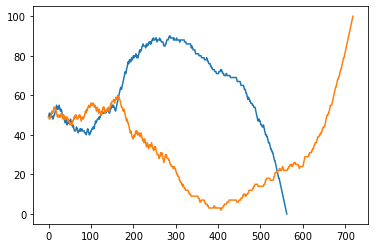
\includegraphics{figures/IMG_ch8/pow1N100mu10}
\caption{$\alpha = 1$, $N = 100$, $\mu = 10$. Two realisations of the process. The reversal can clearly been seen in each case.}
\label{2runs}
\end{figure} 

\subsection*{Results}
Running simulations of the model, for now with $\alpha = 1$, we see that the dynamics can indeed resemble what was observed by Pimentel. Both of the two realisations in figure \ref{2runs} display the same kind of behaviour: after some light initial back and forth, one of the populations grows to a position of significant advantage. But it doesn't last. Trained for intraspecific competition, the oppressed population makes a striking comeback, completely overthrowing their adversaries.\par
This was also observed in the experiment; Blowflies come out on top despite initially being pushed to the brink.\\



\noindent
During the last couple of cycles, before fixation, population counts edge ever so close to the boundary. Here, like with the initially critical poise of Fig. \ref{nodisp2runs}, there is a balance between directive forces; resistance of the comparatively supressed population grows to such an extent that the heavy advantage of their adversaries, is muted. And in this arrived at state of poised criticality, like in the previous case, we see a divergence. The two trajectories, as expected, begin to be swayed by subtle underlying disturbances of stochastic undulations.


\begin{figure}[]
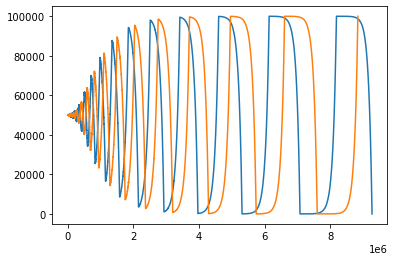
\includegraphics{figures/IMG_ch8/pow10N10e5mu1 2 runs 20e3 no displacement}
\caption{$\alpha = 10$, $N = 10\mathrm{e}5$, $\mu = 1$.  Notice that when the two populations start out well-matched, two parallel realizations of the model diverge more substantially than when the initial state involves a bias. Here we see exactly that. The orange and blue lines represent two different stochastic simulations of the model. Because they begin near the critical region of the model, the future trajectory is much more influenced by the cumulative effect of those initial stochastic influences than might otherwise be the case. In the plot below, you can see a red line depicting the critical zone of the model over time. Being near this line is analogous, in deterministic modeling, to having a high Lyapunov exponent.}
\label{nodisp2runs}
\end{figure} 


\begin{figure}[]
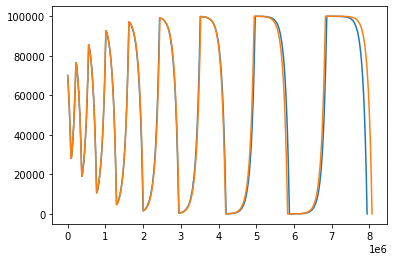
\includegraphics{figures/IMG_ch8/pow10N10e5mu1 2 runs 20e3 displacement}
\caption{$\alpha = 10$, $N = 10\mathrm{e}5$, $\mu = 1$.  As mentioned in the caption of the figure above, when trajectories are started with a bias (one species in the majority), repeated simulations will generally stay closer for longer, only diverging near times of extinction. The critical region plays a role in amplifying small differences in stochastic unfolding.}
\label{disp2runs}
\end{figure} 

To get a more clear understanding of what's really going on here we can actually quantify and map this position of criticality over the course of an experiment. By definition, the system is poised at such criticallity exactly when the likelyhood of making a step up vs down is identical:

\begin{equation*}
q_a = \frac{i_c}{N}(1 - p_b) = \left(1 - \frac{i_c}{N}\right) (1 - p_a) = q_b
\end{equation*}
$i_c$ representing the system state at which there is criticality. From this, taking the fact into consideration that $p_a$ and $p_b$ are non-zero with mutual exclusivity, we can derive the relation: 

$$
i_c = 
\begin{cases}
N\dfrac{1 - p_a}{2 - p_a}, &\text{ when } p_a > 0 \text{ and } p_b = 0  \\
N\dfrac{1}{2 - p_b}, &\text{ when } p_b > 0 \text{ and } p_a = 0 \\
\end{cases}
$$

Bearing in mind that $p_a$ and $p_b$ depend on $R_a$ \& $R_b$, and that these are computed as realisations in a stochastic process, the above formulae are not as analytic as they seem. That being said, it is quite straightforward to generate step by step values of the critical state $i_{c, t}$ computationally. These are visible in red over the standard trajectory of the model in figure \ref{redone}. 




\begin{figure}[H]
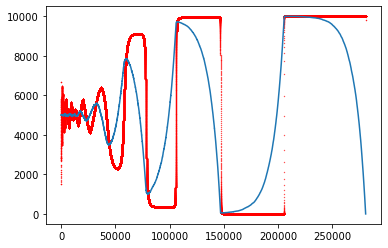
\includegraphics{figures/IMG_ch8/pow3N10e4mu1 critical}
\caption{$\alpha = 3$, $N = 10\mathrm{e}4$, $\mu = 1$. The changing critical saddle is depicted in red. When trajectories are close to this line, small perturbations take on a greater significance.}
\label{redone}
\end{figure} 

If we make a qualitative comparrison beteen whats going on in figure \ref{redone}, and in figures \ref{nodisp2runs} \& \ref{disp2runs}, we can see quite clearly, that in \ref{nodisp2runs} \& \ref{disp2runs} trajectories have a propensity to diverge from one another ecaxtly when the state $A_t$ is near criticality.\par
This toughes the essence of what these notes have been trying to get at: near criticality, the future of a system becomes sensitive, succeptible, light underlying stochastic influences. 


\subsection*{Cellular automaton visualisation}

After formulating the model analytically (note: a model has previously been proposed,  \cite{pease1984evolutionary} but the above model wasn't inspired by this and differs in form),  I thought it would be a good idea to produce a spatial version in the form of a sellular automaton. You can see the results of this is the figure here. Blue and red squares represent houseflies and blowflies respectively. This was coded in C++ using the SFML (Simple fast media layer) library which does low-level graphics. 



\begin{figure}[H]
    \centering
    % First row of four images
    \begin{subfigure}{0.22\textwidth}
        \centering
        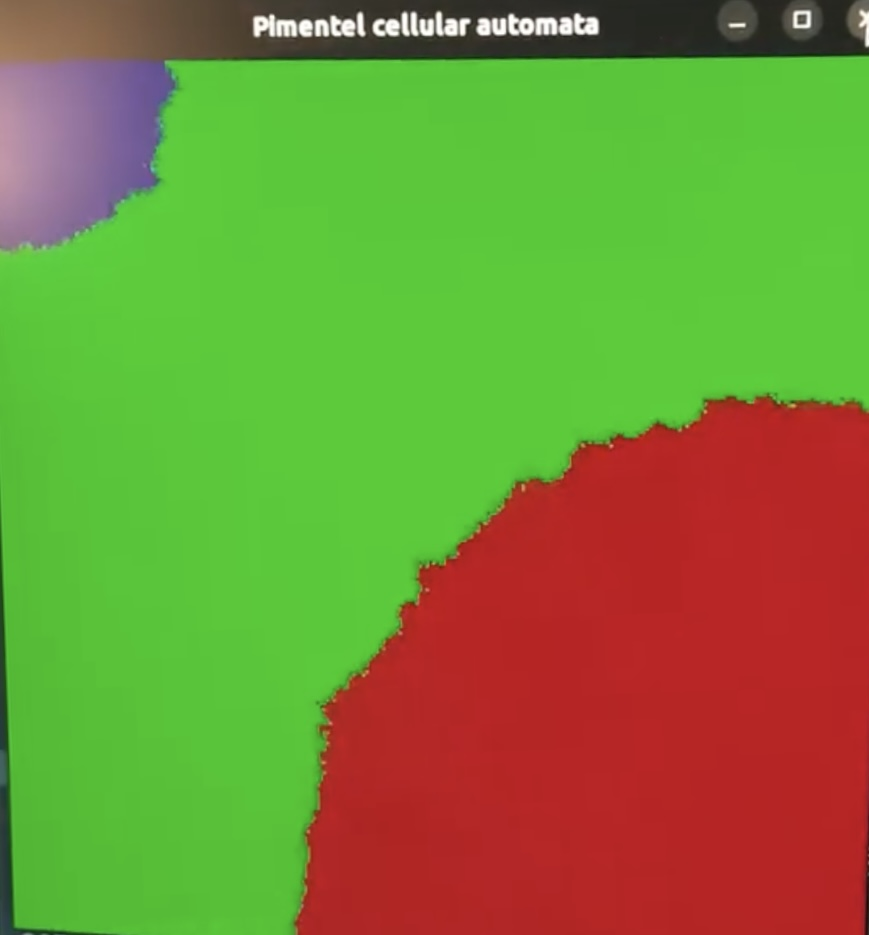
\includegraphics[width=\textwidth]{figures/IMG_ch8/pims/pim1.jpg}
    \end{subfigure}
    \hspace{\fill}
    \begin{subfigure}{0.22\textwidth}
        \centering
        
\includegraphics[width=\textwidth]{figures/IMG_ch8/pims/pim2.jpg}
    \end{subfigure}
    \hspace{\fill}
    \begin{subfigure}{0.22\textwidth}
        \centering
        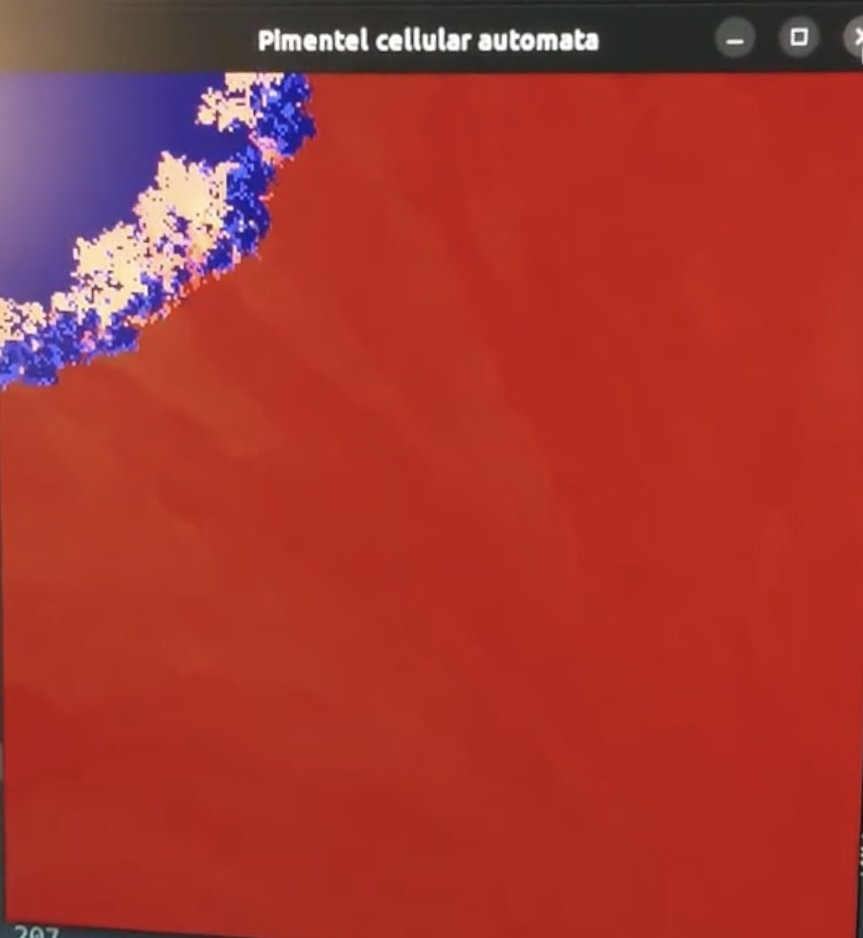
\includegraphics[width=\textwidth]{figures/IMG_ch8/pims/pim3.jpg}
    \end{subfigure}
    \hspace{\fill}
    \begin{subfigure}{0.22\textwidth}
        \centering
        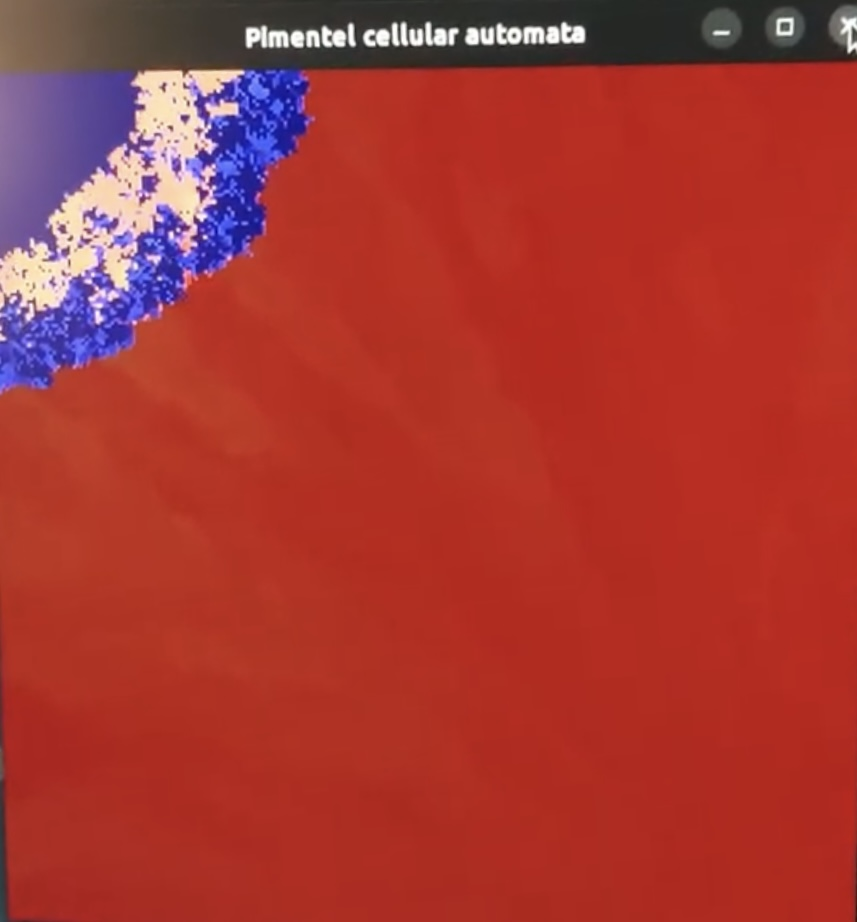
\includegraphics[width=\textwidth]{figures/IMG_ch8/pims/pim4.jpg}
    \end{subfigure}
    
    \vspace{0.5em} % Small vertical space between rows

    % Second row of four images
    \begin{subfigure}{0.22\textwidth}
        \centering
        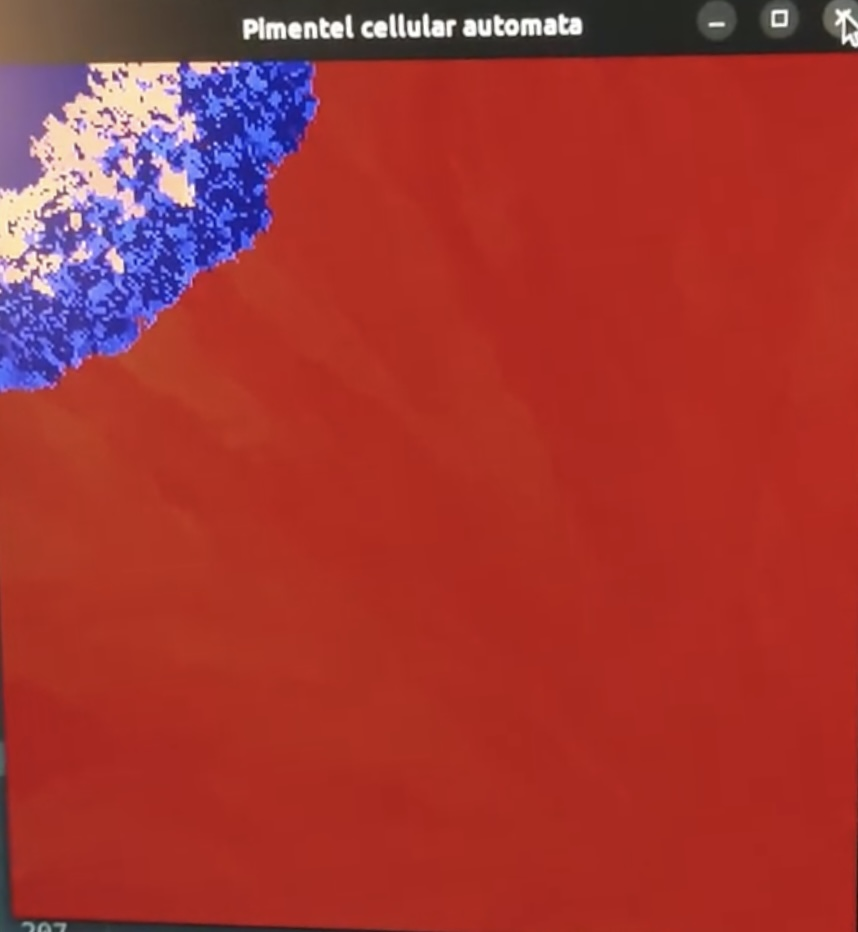
\includegraphics[width=\textwidth]{figures/IMG_ch8/pims/pim5.jpg}
    \end{subfigure}
    \hspace{\fill}
    \begin{subfigure}{0.22\textwidth}
        \centering
        
\includegraphics[width=\textwidth]{figures/IMG_ch8/pims/pim6.jpg}
    \end{subfigure}
    \hspace{\fill}
    \begin{subfigure}{0.22\textwidth}
        \centering
        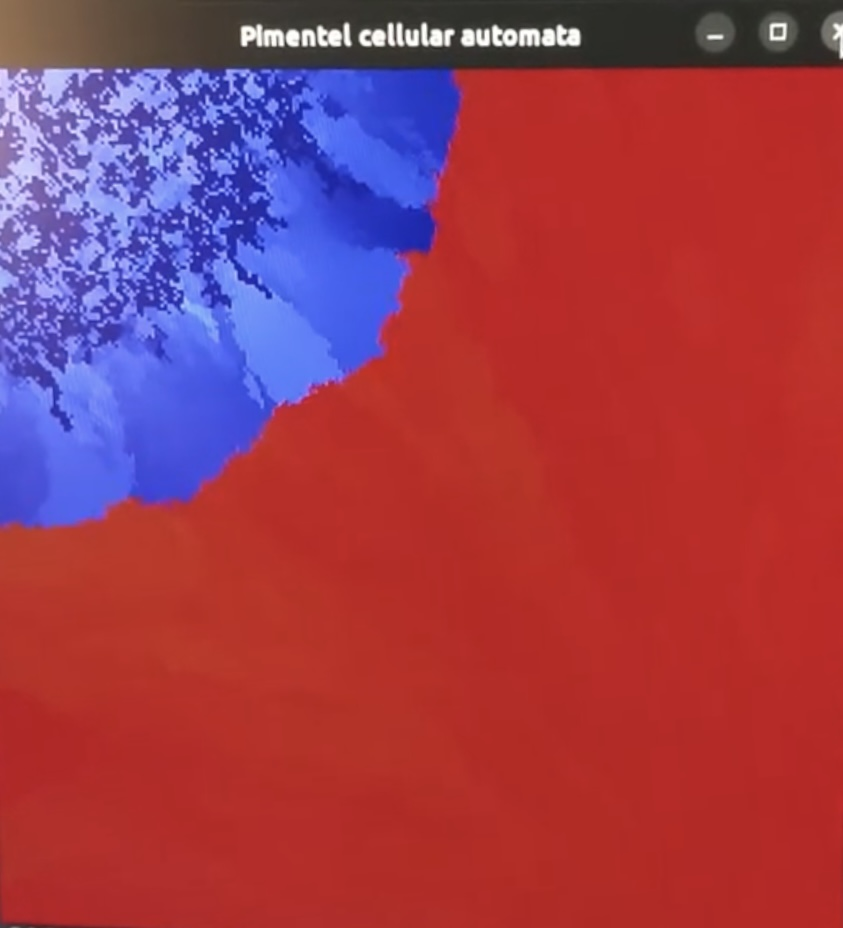
\includegraphics[width=\textwidth]{figures/IMG_ch8/pims/pim7.jpg}
    \end{subfigure}
    \hspace{\fill}
    \begin{subfigure}{0.22\textwidth}
        \centering
        
\includegraphics[width=\textwidth]{figures/IMG_ch8/pims/pim8.jpg}
    \end{subfigure}

    \vspace{0.5em} % Small vertical space between rows

    % Third row of three images
    \begin{subfigure}{0.22\textwidth}
        \centering
        
\includegraphics[width=\textwidth]{figures/IMG_ch8/pims/pim9.jpg}
    \end{subfigure}
    \hspace{10pt}
    \begin{subfigure}{0.22\textwidth}
        \centering
        
\includegraphics[width=\textwidth]{figures/IMG_ch8/pims/pim10.jpg}
    \end{subfigure}
     \hspace{10pt}
    \begin{subfigure}{0.22\textwidth}
        \centering
        
\includegraphics[width=\textwidth]{figures/IMG_ch8/pims/pim11.jpg}
    \end{subfigure}

    % Single caption for all images
    \caption{Picured above is a series of frames from an animation: a spatial cellular automaton version of the pimental model. You can see that the initial advantage of the red population is cast aside by the blues after they become hardened and more competetive following intraspecific interactions. The shades within each population only depict relative heredity and don't have any bearing on the dynamics. }
    \label{fig:sequential_images}
\end{figure}



\subsection{Pimental +}


\noindent
It might be possible to use the pimental model to frame a description of a hypothetical link between speciation and population collapse. An endogeneous process in which the unleasing of variation (facilitated by favourable conditions), can ultimately lead to the demise of a population, as other groups rise to dominance. This process is an attempt to mathematisize what Nietzcche described alegorically in words: the process by which group variation results from favourable circumstances, but how this itself can lead to failiure through a weakining of established forms. The following quote is from``Beyond good and evil'' section 262 \cite{nietzsche2013beyond}:


\begin{quotation}
``A species originates, and a type becomes established and strong in the long struggle with
essentially constant unfavourable conditions. On the other hand, it is known by the experience of
breeders that species which receive super-abundant nourishment, and in general a surplus of
protection and care, immediately tend in the most marked way to develop variations, and are
fertile in prodigies and monstrosities (also in monstrous vices). Now look at an aristocratic
commonwealth, say an ancient Greek polis, or Venice, as a voluntary or involuntary contrivance
for the purpose of rearing human beings; there are there men beside one another, thrown upon
their own resources, who want to make their species prevail, chiefly because they must prevail,
or else run the terrible danger of being exterminated. The favour, the super-abundance, the
protection are there lacking under which variations are fostered; the species needs itself as
species, as something which, precisely by virtue of its hardness, its uniformity, and simplicity of
structure, can in general prevail and make itself permanent in constant struggle with its
neighbours, or with rebellious or rebellion-threatening vassals. The most varied experience
teaches it what are the qualities to which it principally owes the fact that it still exists, in spite of
all Gods and men, and has hitherto been victorious: these qualities it calls virtues, and these
virtues alone it develops to maturity. It does so with severity, indeed it desires severity; every
aristocratic morality is intolerant in the education of youth, in the control of women, in the
marriage customs, in the relations of old and young, in the penal laws (which have an eye only
for the degenerating): it counts intolerance itself among the virtues, under the name of "justice."
A type with few, but very marked features, a species of severe, warlike, wisely silent, reserved,
and reticent men (and as such, with the most delicate sensibility for the charm and nuances of
society) is thus established, unaffected by the vicissitudes of generations; the constant struggle
with uniform unfavourable conditions is, as already remarked, the cause of a type becoming
stable and hard. Finally, however, a happy state of things results, the enormous tension is
relaxed; there are perhaps no more enemies among the neighbouring peoples, and the means of
life, even of the enjoyment of life, are present in super abundance. With one stroke the bond and
constraint of the old discipline severs: it is no longer regarded as necessary, as a condition of
existence--if it would continue, it can only do so as a form of luxury, as an archaising taste.
Variations, whether they be deviations (into the higher, finer, and rarer), or deteriorations and
monstrosities, appear suddenly on the scene in the greatest exuberance and splendour; the
individual dares to be individual and detach himself. At this turning-point of history there
manifest themselves, side by side, and often mixed and entangled together, a magnificent,
manifold, virgin-forest-like up-growth and up-striving, a kind of tropical tempo in the rivalry of
growth, and an extraordinary decay and self-destruction, owing to the savagely opposing and
seemingly exploding egoisms, which strive with one an other "for sun and light," and can no
longer assign any limit, restraint, or forbearance for themselves by means of the hitherto existing
morality. It was this morality itself which piled up the strength so enormously, which bent the
bow in so threatening a manner:--it is now "out of date," it is getting "out of date." The
dangerous and disquieting point has been reached when the greater, more manifold, more
comprehensive life is lived beyond the old morality; the "individual" stands out, and is obliged to
have recourse to his own law-giving, his own arts and artifices for self-preservation, self-
elevation, and self-deliverance. Nothing but new "Whys," nothing but new "Hows," no common
formulas any longer, misunderstanding and disregard in league with each other, decay,
deterioration, and the loftiest desires frightfully entangled, the genius of the race overflowing
from all the cornucopias of good and bad, a portentous simultaneousness of Spring and Autumn,
full of new charms and mysteries peculiar to the fresh, still inexhausted, still unwearied
corruption. Danger is again present, the mother of morality, great danger; this time shifted into
the individual, into the neighbour and friend, into the street, into their own child, into their own
heart, into all the most personal and secret recesses of their desires and volitions. What will the
moral philosophers who appear at this time have to preach? They discover, these sharp onlookers
and loafers, that the end is quickly approaching, that everything around them decays and
produces decay, that nothing will endure until the day after to-morrow, except one species of
man, the incurably mediocre. The mediocre alone have a prospect of continuing and propagating
themselves--they will be the men of the future, the sole survivors; "be like them! become
mediocre!" is now the only morality which has still a significance, which still obtains a hearing.--
But it is difficult to preach this morality of mediocrity! it can never avow what it is and what it
desires! it has to talk of moderation and dignity and duty and brotherly love--it will have
difficulty in concealing its irony!''
\end{quotation}

The basic pimental model as defined above encorporates the fitness of two populations, these increasing when the particular species is pushed into a minority. 

$$\pr{\Delta A_t = 1} = \frac{A_t}{N} \frac{f_a}{\bar f}$$

$$\pr{\Delta A_t = 1} =\lrb{ 1 - \frac{A_t}{N}} \frac{f_b}{\bar f}$$




where $A_t$, $B_t$, and $N$ represent the relative domination of group $A$, group $B$, and the total domain capacity. With the Moran assumption, $A_t = N - B_t$. Like above, these are essentially the probabilities of a chosen individual encountering a member of the opposite group ($A_t/N$) \textbf{and} defeating them in competition ${f_a}/{\bar f}$. In this unaltered model, fitness changes according to

$$f_a(t+\Delta t) = f_a(t) + \delta \lrb{\frac{B_t}{A_t}}^\alpha$$

$$f_b(t+\Delta t) = f_b(t) + \delta \lrb{\frac{A_t}{B_t}}^\alpha$$

\noindent
Note: this is a slightly different definition to the one shown above. $R_a$ \& $R_b$ are replaced by $f_a$ \& $f_b$, but the dynamics are at least qualitativaly identical. 

\subsubsection*{Sub-species, including variable speciaton}

Suppose we incorporate a species count for each population, $\xt^{(a)}$ and $\xt^{(b)}$, respectively. According to the alagory laid out by neitche, exxessive variation (the emergence of many species), leads to a weakening of a population. In our model, that would be represented by a drop in fittness. But how does the number of species change. Generally speaking, variation will increase when the demands of survival are lessened by favourable circumstances. In our model, something like this will be represented by the product of domain control and fitness.\par 
Take for example

$$\pr{\Delta \xt^{(a)} = 1}  = \beta_a\xt^{(a)} \Delta t$$

$$\pr{\Delta \xt^{(a)} = -1}  = \mu_a\xt^{(a)} \Delta t$$

\noindent
with extinction $\mu_a$ constant, and speciation $\beta_a$ varing according to fitness, $f_a$, and relative domination $(A_t / N)$:

$$\beta_a = \lrb{\frac{A_t}{N}}^\lambda f_a$$ 

\noindent
The dynamics for the other species count $\xt^{(b)}$ would function in the same way but with $A_t$ being replaced by $B_t$ etc... 

\subsubsection*{Effect of species count on fitness}

\noindent
Then there is the effect of excess variation on reducing a group's fitness.Something like this could serve well,

$$f_a(t+\Delta t) = f_a(t) + \delta \lrb{\frac{B_t}{A_t}}^\alpha  - \gamma \xt^{(a)}$$

$$f_b(t+\Delta t) = f_b(t) + \delta \lrb{\frac{A_t}{B_t}}^\alpha  - \gamma \xt^{(b)}$$

\noindent
with constant $\gamma$ representing the abount by which the inneficencies of excess variations weigh on overall performance. \par 

\subsubsection*{Comments}
Unfortunately, for this model, along with half a dozen other speculative models relating to speciation and evolution, I didn't get round to running simulations or doing much analysis. This is inevitable. and the model outlined here is itself a description of why. Models, like any other form of coded information are subject to the laws of variation whereby one model, on creative consideration, soon gives birth to many more. And with time and energy resources being limited, a multiplicity like this hs the effect of spreading resources more thinly, each gets less and less attention as the number increases. And before you know it, its time to write a thesis, and most of them get discarded.\par
But I thought, I'd at least write this one down, because it contains my best attempt at describing mathematically the endogeneous aspect of collapse by variation.
